% This must be in the first 5 lines to tell arXiv to use pdfLaTeX, which is strongly recommended.

% In particular, the hyperref package requires pdfLaTeX in order to break URLs across lines.

\documentclass[11pt]{article}
\pdfoutput=1
% Remove the "review" option to generate the final version.
\usepackage{ACL2023}
\usepackage{caption}
% Standard package includes
\usepackage{times}
\usepackage{latexsym}
\usepackage{graphicx}
\usepackage{amsmath}
% For proper rendering and hyphenation of words containing Latin characters (including in bib files)
\usepackage[T1]{fontenc}
% For Vietnamese characters
% \usepackage[T5]{fontenc}
% See https://www.latex-project.org/help/documentation/encguide.pdf for other character sets

% This assumes your files are encoded as UTF8
\usepackage[utf8]{inputenc}

% This is not strictly necessary, and may be commented out.
% However, it will improve the layout of the manuscript,
% and will typically save some space.
\usepackage{microtype}

% This is also not strictly necessary, and may be commented out.
% However, it will improve the aesthetics of text in
% the typewriter font.
\usepackage{inconsolata}


% If the title and author information does not fit in the area allocated, uncomment the following
%
%\setlength\titlebox{<dim>}
%
% and set <dim> to something 5cm or larger.

\title{Comparative Study of Binary Sentiment Analysis for the Product Review dataset with the Explainable AI framework} 

\author{Dimitra Muni\\
  732A92 - Text Mining \\
  Linköping University \\
  \texttt{dimmu472@student.liu.se}
  }
\begin{document}

\maketitle
\begin{abstract}
This project aimed to analyze binary sentiment for the Amazon Fine Food Reviews dataset\footnote{\url{https://snap.stanford.edu/data/web-FineFoods.html}} using different vectorization and word embedding techniques and evaluated the performance on the gold standard dataset. In the first part of the project, we utilized two different word vectorization (i.e. count  and TF-IDF vectorizers) techniques in conjunction with three linear classifiers (i.e. Multinomial Naive Bayes, Logistic Regression, and Support Vector Machine (SVM) ) to create six experimental pipelines. Furthermore, we used the \textit{Halving Grid Search} technique to find the best-performing model with five-fold cross-validation. Here SVM slightly outperformed the other two models with an accuracy of 93\%. In the second part of the project, we utilized four pre-trained compact BERT models and DistilBERT to perform sentiment classification on a smaller subset of original data; as expected, DistilBERT outperformed the other compact BERT models, however, as it was not tuned on the entire training data, the performance was not as high as SVM model. In the third part of the project, we performed LIME \cite{LIME} analysis for a subset of misclassified samples identified from the final SVM model and documented actionable insights.
\end{abstract}

\section{Introduction}
In the last decade, massive development in Masked Language Models has opened the floodgates of possibility in Natural Language Processing (NLP) domain. 
\textbf{B}idirectional \textbf{E}ncoder \textbf{R}epresentations from \textbf{T}ransformers (BERT), developed by \cite{BERT} at Google, is one such model. The base version of BERT has 110 million parameters and is computationally expensive to train. Several variants of this model, such as DistilBERT \cite{distilbert} and a compact version of BERT developed by \cite{smallBERT}, are significantly faster than the base version of BERT; however, with a decline in performance.

These models can be utilized to address several different tasks, such as machine translation, context disambiguation, named entity recognition (NER), and sentiment analysis, to name a few. In this project, we focus on the problem of binary sentiment analysis for the Amazon Fine Foods dataset, which contains product reviews collected over a decade. We intend to address the following research objectives,
\begin{enumerate}
    \item Experiment with word vectorizer-based technique with machine learning classifiers to perform sentiment classification.
    
    \item Investigate the applicability of the compact Masked Language Models (MLMs) for sentiment classification.
    
    \item Inference about misclassified samples obtained from the best-performing model, generating actionable insight using an explainable AI technique.
\end{enumerate}
In the initial part of this project, we performed data cleaning and pre-processing on the Amazon Fine Foods dataset, which contains reviews with scores from 1 to 5. In the pre-processing part, the original dataset was converted into a smaller dataset with two classes, i.e. positive and negative reviews; we elaborate on this in the later stage. Next, we split the reduced dataset into training and test sets with an 85\%-15\% split. We use the test set only for the evaluation in the later stage. As the training set had a class imbalance, we performed random down-sampling to create a balanced training set. 

Next, we created six different vectorizer-classifier pipelines, using two vectorizers and four classifiers; we utilized a halving grid search technique with five-fold cross-validation to tune these pipelines and evaluated the performance on the test set.

In the second part of the project, we use transformer-based embedding using five small BERT models with different numbers of transformer blocks and hidden layer size combinations; we trained the model for ten epochs and evaluated the performance on the test set. Next, we repeated this process for the DistilBERT model. In our experiments, we utilized Tensorflow Hub to utilize these models.

 In the last part of the project, we focus on the misclassified samples (from the test set) identified using the Linear SVM model. We used a popular explainable AI technique called LIME analysis \cite{LIME} to perform this study.

 \section{Theory}
\subsection{Vectorization}
The vectorization technique converts the corpus of text data into a matrix representation; one such technique is Count Vectorizer, which uses a \textit{bag-of-word} representation \cite{jurafsky}. Here the corpus is assumed to be a collection of words, where a matrix represents the frequency of the word \textit{w} in document \textit{d}. One noteworthy constraint of this representation is that the word's position in a sentence is not inconsequential; rather, the frequency of the word is important \cite{jurafsky}. 
Another more advanced method of vectorization is \textit{TF-IDF}; here, \textbf{TF} refers to the \textbf{term frequency}, which accounts for the occurrence of the term \textit{t} in document \textit{d}, while \textit{idf} is \textbf{inverse document frequency}, a measure of the number of documents a term \textit{t} appears. Here in the equation [\ref{eq:tfidf}], the inverse document frequency of term t ($idf_t$) is calculated on the logarithm scale, where \textit{n} is the total number of documents.
\begin{equation}
\label{eq:tfidf}
\small
\begin{aligned}
w_{t,d}&=tf_{t,d} \times idf_{t}\\
tf_{t,d}&=count(t,d)\\
idf_{t}&=\ln \left(\frac{1+n}{1+ df_t}\right)+1   
\end{aligned}    
\end{equation}
There are several variations in the way $tf_{t,d}$, and $idf_t$ are calculated, but we choose this definition [\ref{eq:tfidf}] to be consistent with the default settings of the \texttt{sklearn} library \texttt{TfidfVectorizer} implementation. One noteworthy advantage of TF-IDF representation is that it assigns relevance to rare occurring words by higher IDF value \cite{info-ret}.

\subsection{Classifiers}
\subsubsection{Multinomial Naive Bayes}
Multinomial Naive Bayes classifier is based on Bayes' rule \cite{bayes}\footnote{Bayes' rule for two events x and y is presented as in term of conditional probability, $p(x|y)p(y)=p(y|x)p(x)$.} about the conditional probability of two events. This classifier is often a preferred  baseline evaluation method due to its simplicity. According to Jurafsky and Martin (p.61, 2023), there is a \textbf{naive} assumption about conditional independence of the feature probability given the class ($P(f_i|c)$); the authors represented this mathematically as,   
\begin{equation}
\small 
\label{eq:MNB-1}
c_{NB} = \underset{c\in C}{\mathrm{argmax}} 
\, P(c) \underset{f \in F}{\prod}P(f|c)
\end{equation}
Here $P(c)$ is the prior probabilities of each class $c$ (where $c \in C$), whereas $f$ is a feature that refers to the word in the document. Authors represented equation [\ref{eq:MNB-1}] in terms of log scale [\ref{eq:MNB-2}] for efficient computation.
\begin{equation}
  \label{eq:MNB-2}
  \small
  c_{NB}=\underset{c\in C}{\mathrm{argmax}} \left(log(P(c))+ \sum_{i\in positions}log(P(w_i|c))\right)
\end{equation}
Here $P(w_i|c)$ is the probability of a word at $i^{th}$ location while conditioning on class c, $P(c)$ and $P(w_i|c)$ were represented as,

\begin{equation}
\label{eq:MNB-3}
\small
P(c)=\frac{N_c}{N_{doc}};P(w_i|c)=\frac{count(w_i,c)+\alpha}{(\sum_{w \in V}count(w,c))+\alpha |V|}
\end{equation}
In the equation [\ref{eq:MNB-3}], $N_c$ is the number of documents from the dataset with class c. $N_{doc}$ represents the total number of documents in the dataset. $|V|$ is the size of vocabulary V, which comprises all the words in the corpus. $\alpha$ is the smoothing parameter ($\alpha \ge 0$), which adds the extra occurrence of words to prevent zero probability. If the $\alpha=0$, then there is no smoothing applied. Usually, this parameter is optimized using validation data. 

\subsubsection{Logistic Regression}
According to Bishop and Nasrabadi (p.205, 2006), the logistic regression classifier is one of the linear classifier models that uses \textit{logistic sigmoid} function\footnote{logistic sigmoid: $\sigma(a)=\frac{1}{1+\exp{(-a)}}$} for binary classification and attempts to minimize \textbf{cross-entropy loss}. 
Jurafsky and Martin (p.86, 2023)
asserted that for the correlated features, the logistic regression classifier is preferred over naive Bayes because the logistic regression can assign the weights more efficiently amongst the correlated features; while this mechanism is not present in the naive Bayes model; due to this reason, we intend to use this model in our experiments. However, this model has a disadvantage that, as it uses the gradient descent method to update its weight, it usually takes longer time to train.

Now, we refer to the documentation of the logistic regression model (\texttt{LogisticRegression} function) in the \texttt{sklearn} library\footnote{\url{https://scikit-learn.org/stable/modules/linear_model.html\#logistic-regression}}, where the optimization problem is formulated as:
\begin{equation}
\label{eq:lr}
\scriptsize \underset{w}{min}\left( C\sum_{i=1}^n \left(y_i \log(P(X_i)) - (1-y_i) \log(1-P(X_i))\right)  + r(w)  \right)
\end{equation}
Here, $y_i$ is the binary target value, $X_i$ represents the input feature for the sample $i$, and $w$ is the corresponding weight. Furthermore, $r(w)$ refers to the \textit{penalty} term that controls the model's regularization. In our baseline experiments, we do not use any \textit{penalty} but rather tune the regularization term \textit{C}.

\subsubsection{Support Vector Machines}
Support Vector Machine (SVM) classifier originally presented by \cite{vapnik} belongs to the class of \textit{maximum margin classifiers} \cite{bishop}, where the objective is to find a hyperplane that separates two classes with the highest margin. There are several variations of SVM classifiers based on the kernel function. However, we only consider the Linear SVM classifier, using the \texttt{LinearSVC} function from \texttt{sklearn} library; we refer to the documentation\footnote{\url{https://scikit-learn.org/stable/modules/svm.html\#support-vector-machines}}, where the problem is formulated as follows:
\begin{equation}
\small
   \underset{w,b}{min} \left(\, \frac{1}{2}||w||^2 + C \sum_{i=1}^n max(0,1-y_i(w^T\phi(x_i)+b))\right)\\
\end{equation}
This classifier utilizes \textbf{hinge loss} described by $max(0,1-y(w^T \phi(x)+b))$. Here $x_i$ is the training vector, $y_i$ is the vector with value $\{-1,1\}$. $\phi$ is the identify function\footnote{Identitiy function, $f(X)=X$}. $C$ is the term that controls the regularization (similar to that in Logistic Regression, $w$ is the weight vector. SVM classifier finds the maximum margin between support vectors by minimizing the $||w||^2$. According to the \href{https://scikit-learn.org/stable/modules/svm.html#support-vector-machines}{documentation} for SVM, this method is appropriate for datasets with high dimensions if the dataset has considerably more samples ($n>>p$) than the number of features, for this reason, we include this method in our analysis.

\subsection{Masked Language Models}
According to \cite{BERT}, the BERT model is trained using a \textit{masked language modeling} technique, where a model is trained by hiding randomly chosen tokens and is asked to predict that token. This model introduces bidirectional context to the training of transformer-based architecture using the attention mechanism \cite{attention}. The BERT model is trained in two iterations; the first iteration is called \textbf{pre-training}, where the model is trained on unlabeled data, and the second is \textbf{fine-tuning}, where the model is tuned on labeled data. 

The BERT-base model has 12 transformer blocks, with a hidden size of 768 and 12 attention heads. This model uses WordPiece embedding \cite{wordpiece}, which converts a word into sub-word units.

In figure [\ref{fig:BERT_archi}], the pre-training and fine-tuning procedure is represented, where a sentence pair is separated by \texttt{[SEP]} token, and before each sentence, there is a classification token \texttt{[CLS]}. Input embedding is denoted by \textbf{\textit{E}}, and \textbf{\textit{C}} represents the final vector corresponding to \texttt{[CLS]} token, and $T_1, T_2, ..., T_N$ represents tokens' final vector representation, where \textit{N = 768} for the BERT-base model.  

According to \cite{BERT}, BERT is pre-trained on two tasks; the model is trained to predict the masked words in the first \textit{Masked Language Modelling} task, where 15\% of tokens are chosen at random and masked. Furthermore, out of these 15\% tokens, 80\% tokens are masked with \texttt{[MASK]} token, 10\% are replaced with a random token, and 10\%  of tokens remain unchanged. The second task is \textit{Next Sentence Prediction (NSP)}, where the model is trained by evaluating whether a sentence is followed by another sentence, using labels such as \texttt{IsNext} or \texttt{NotNext} for\textit{ Question Answering (QA)} and \textit{Natural Language Inference (NLI)} use cases. In the next stage, the BERT model is fine-tuned on a different dataset based on the corresponding application.

\begin{figure*}
\label{fig:BERT_embedding}
    \centering
    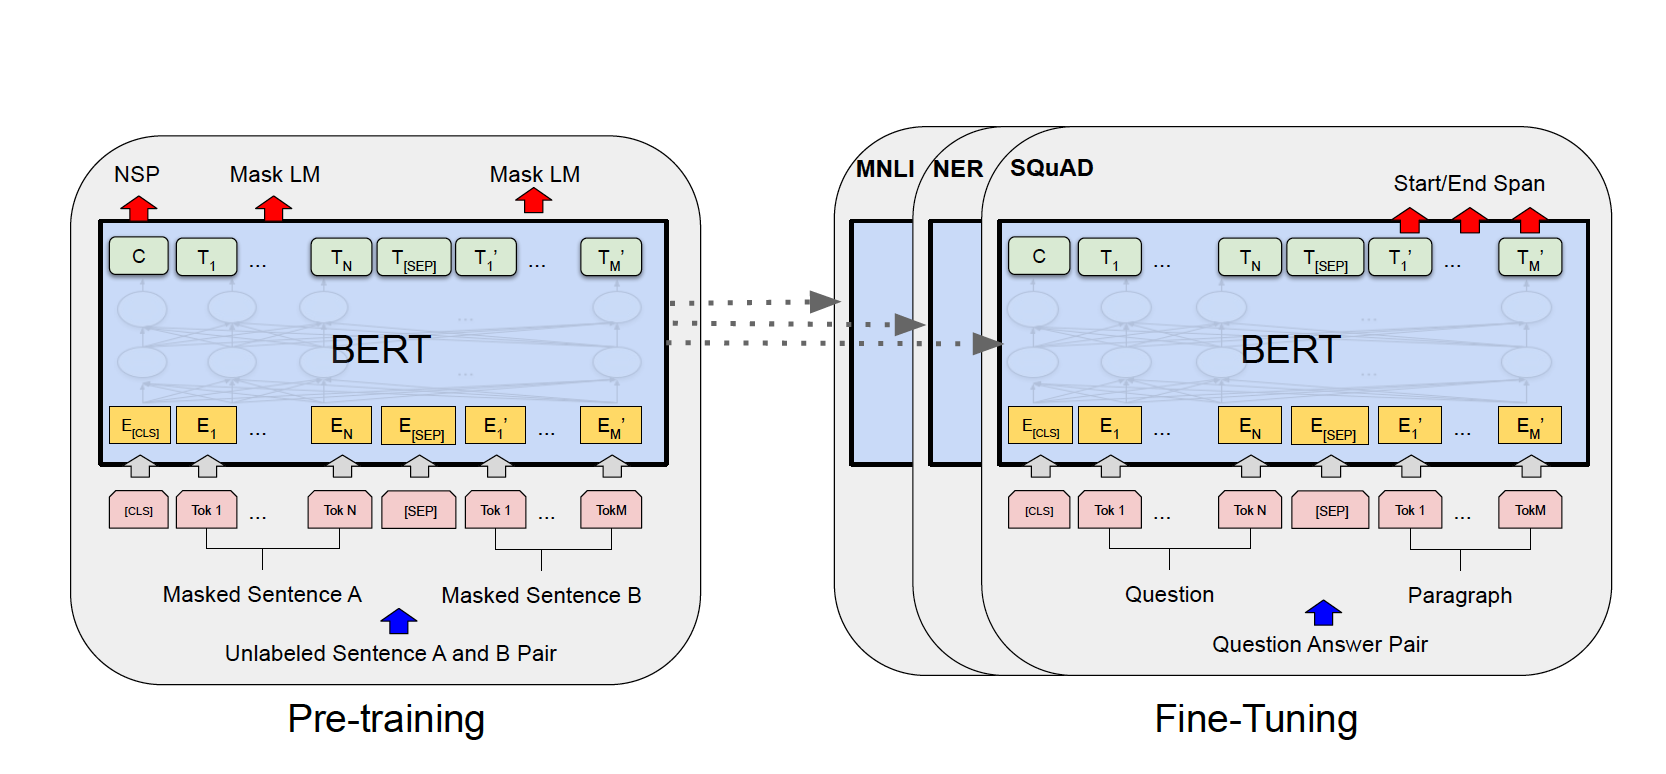
\includegraphics[scale=0.6]{figures/BERT-embedding.png}
    \caption{Pre-training and Fine tuning procedure in BERT, the figure taken from Devlin et al. (p.3, 2019)}
    \label{fig:BERT_archi}
\end{figure*}
One important limitation of the BERT model is the higher computational cost; several compact versions of BERT address this issue, however, with some performance loss.

\subsubsection{Compact Versions of BERT}
The compact version of BERT introduced by \cite{smallBERT} uses the student-teacher paradigm for knowledge distillation. Here the teacher is a large or base BERT model, while the student is a smaller BERT model with fewer parameters, e.g. \textbf{\small BERT-128/2}, which comprises 4.4 million parameters. The authors have presented 24 different models with varying numbers of transformer blocks, hidden embedding sizes, and attention heads. However, we only chose four models as described in table [\ref{tab:sbert_distil}] for the limited scope of this project.

The compact BERT model training procedure is described as \textbf{Pre-trained distillation} in figure [\ref{fig:smallBERT_archi}]. Authors have used three types of datasets in training these models, unlabeled language model data ($\mathcal{D}_{LM}$), unlabeled transfer data ($\mathcal{D}_{T}$), and labeled data ($\mathcal{D}_{L}$). First, using a masked language modeling technique, the compact model is pre-trained on $\mathcal{D}_{LM}$. Next, the large teacher model transfers the knowledge with $\mathcal{D}_{T}$ to the student model in the distillation phase.

According to the author, knowledge distillation is the technique \cite{kdistillation},  where a bigger teacher model transfers the knowledge to a more compact model by producing \textit{soft labels}, which is a probability distribution for class $l$, calculated 
as 
\begin{equation}
\label{eq:softmax-temp}
\small
    p_l=sofmax(z_l/\mathcal{T})
\end{equation}
 Here, $z_l$ is the last embedding layer value (logit) for class $l$, $\mathcal{T}$ is the temperature that can be tuned to smoothen the distribution. In the case of these 24 compact BERT models, the temperature value is chosen to be $\mathcal{T}=1$; because the authors \cite{smallBERT} did not observe an improvement in performance when changing this value of this parameter.
Finally, the compact model is fine-tuned on $\mathcal{D}_{L}$.

\begin{figure}
\label{fig:small_BERT}
    \centering
    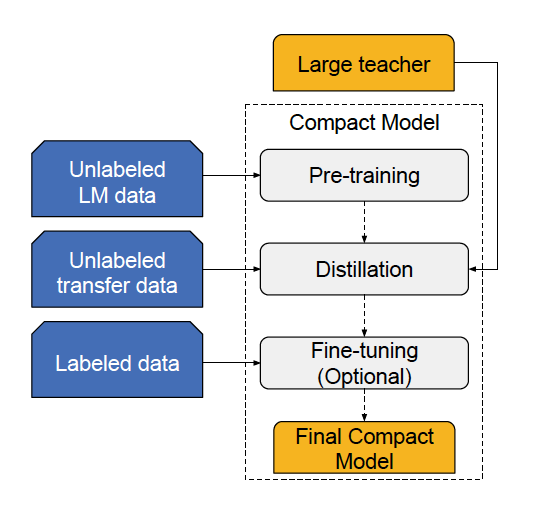
\includegraphics[scale=0.6]{figures/smallBERT.png}
    \caption{Pre-trained Distillation for Compact BERT model, the figure taken from Turc et al (p.2, 2019)}
    \label{fig:smallBERT_archi}
\end{figure}

\subsubsection{DistilBERT}
DistilBERT, introduced by \cite{distilbert}, is another example of a compact model, with the number of layers reduced by half\footnote{Additionally token-type embedding and pooler are removed as well.}, and has a similar architecture to that of a BERT-base model, but  it uses the knowledge distillation technique also used in compact BERT models but employs triple loss function. 
\textbf{Triple Loss:}
Authors trained DistilBERT using a linear combination of three loss functions, cross-entropy distillation loss ($L_{ce}$), masked language modeling loss ($L_{mlm}$), and cosine embedding loss ($L_{cos}$) calculated by performing cosine operation on a hidden vector of student and teacher. Here the distillation loss $L_{ce}$ is calculated as,
\begin{equation}
 \small L_{ce}=\sum_i t_i * log(s_i)
\end{equation}
Here $t_i$ refers to the probabilities by the teacher, while $s_i$ is the probabilities corresponding to student. Here $t_i$ and $s_i$ are calculated using softmax-temperature, described in equation [\ref{eq:softmax-temp}]\footnote{Temperature for student and teacher is the same during training}.


According to \cite{distilbert} \textbf{DistilBERT} is significantly faster (60\%) and smaller (40\%) than BERT-base. The authors evaluated DistilBERT for the sentiment classification task on the IMDb dataset, and it performed almost at par (accuracy of 92.82) with BERT-base (accuracy of 93.46). We intend to investigate the usage of DistilBERT for a similar task but with the Amazon Fine Foods dataset.
\subsection{LIME}
\textbf{L}ocal \textbf{I}nterpretable \textbf{M}odel agnostic \textbf{E}xplanation (LIME) \cite{LIME} is a popular explainable AI framework to understand the underlying pattern that black box models are trained with and for the inference about the predictions. LIME perturbs the black-box model, observes local changes, and provides a visual explanation for greater understanding. LIME is model agnostic, i.e. it can be used for any model and provide explanations.


Another widely used model for this application is SHAP analysis, \textbf{SH}apley \textbf{A}dditive Ex\textbf{P}lanation is an explainable AI framework, which was developed by \cite{shap}\footnote{ SHAP framework is based on the concept of Shapley values, that are used in game theory to assign the credits to participants based on the coalitions formed by them \cite{shapley}}. One notable advantage of LIME over SHAP is that it is relatively faster to model. However, the SHAP framework provides global explanations for the underlying model; this might be paramount in certain use cases where SHAP is the preferred method. 

\subsection{Evaluation Metrics}
Here we present the definition of different evaluation metrics utilized in our analysis. In the table [\ref{tab:confusion_mat}], we demonstrate the terminology associated with the confusion matrix.


\begin{table}
\small
    \centering
    \begin{tabular}{c| c c}
    \hline 
         & \textbf{Predicted True} & \textbf{Predicted False} \\ \hline 
    \textbf{Actual True}  & True Positive (\textbf{TP}) & False Negative (\textbf{FN})\\
    \textbf{Actual False}   & False Positive (\textbf{FP}) & True Negative (\textbf{TN})\\\hline 
         
    \end{tabular}
    \caption{Confusion Matrix}
    \label{tab:confusion_mat}
\end{table}
\subsubsection{Precision}
Precision for the positive class can be calculated as:
\begin{equation}
\small Precision =\frac{TP}{TP+FP}
\end{equation}
Precision for the negative class can be calculated as:
\begin{equation}
\small Precision =\frac{TN}{TN+FN}
\end{equation}
\subsubsection{Recall}
Recall for the positive class can be calculated as:
\begin{equation}
    \small Recall =\frac{TP}{TP+FN}
\end{equation}
Recall for the negative class can be calculated as:
\begin{equation}
    \small Recall =\frac{TN}{TN+FP}
\end{equation}

\subsubsection{F1-score}
F1-score is the harmonic mean of Precision and Recall, which is calculated as follows:
\begin{equation}
\small    F1  = \frac{2\cdot Precision\cdot  Recall}{Precision + Recall}
\end{equation}
\subsubsection{Accuracy}
Accuracy for a given model can be computed using the following equation,
\begin{equation}
    \small Accuracy = \frac{TP+TN}{TP+TN+FP+FN}
\end{equation}
 \section{Data}
 \label{sec:data}
 We have chosen the Amazon Fine Foods dataset hosted on the \href{https://snap.stanford.edu/about.html}{SNAP library} affiliated with Stanford University. This dataset contains reviews of 74,258 unique products and 568,454 product reviews by 256,059 users, collected between October 1999 and October 2012.
 
 The features of this dataset are described in the table [\ref{feat-description}].
 \begin{table}
    \centering
     \begin{tabular}{c c}
     \hline
          \textbf{Feature} & \textbf{Description}\\ \hline 
     productId &\href{https://en.wikipedia.org/wiki/Amazon_Standard_Identification_Number}{ASIN} - Amazon Standard \\
     & Identification Number\\ \hline
          userId & reviewer identification \\
          profileName & reviewer profile name\\
          helpfullness & fraction of users\\
          & who found the review helpful\\
          score & score from 1 to 5\\
          time &time of review post\\
          summary&review summary \\ 
          text & review text\\   \hline
     \end{tabular}
     \caption{Feature Description for Amazon Fine Food dataset}
     \label{feat-description}
 \end{table}
 Our analysis focused on the \textit{text} and \textit{score} variables. Firstly, in figure [\ref{fig:review_score_distri}], the distribution of review score is presented, where the dataset had a class imbalance, with a higher number of reviews with a score of 5. 
\begin{figure}
     \centering
     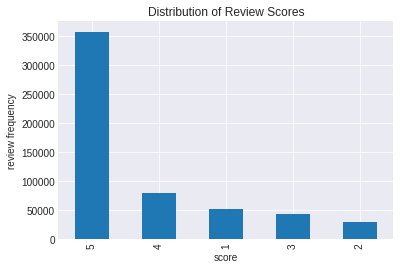
\includegraphics[scale=0.5]{figures/distribution_review_score.png}
     \caption{Distribution of Review Scores}
     \label{fig:review_score_distri}
 \end{figure}
 Secondly, in figure [\ref{fig:review_score_wordlength}], the mean number of words for review ranges from 70 to 87; interestingly, the reviews that have scored 5 tend to be shorter comparatively than the other four classes of reviews.
 \begin{figure}
     \centering
     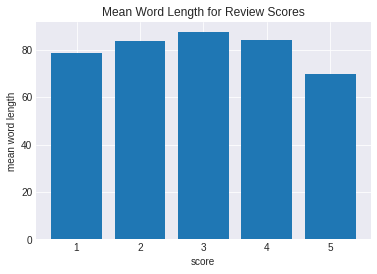
\includegraphics[scale=0.5]{figures/mean_wordlength_distribution.png}
     \caption{Distribution of mean of the number of words per review score}
     \label{fig:review_score_wordlength}
 \end{figure}
  \begin{table}[h!]
 \small
     \centering
     \begin{tabular}{c| c c | c c}
     \hline 
        Type & Positive & Negative &Positive &Negative\\ \hline 
         Train &  371989 &68965 &68965 & 68965\\
          Test & 65646 &12170 & 65646 &12170\\ \hline 
     \end{tabular}
     \caption{Distribution of Positive and Negative Class before and after Undersampling}
     \label{tab:class_distri}
 \end{table}
 As we intend to perform a binary classification of the review dataset, the newly engineered dataset disregards the reviews with a score of 3, and the reviews with scores 1 and 2 are encoded with binary value '1' and reviews with scores 4 and 5 are encoded with '0'. After performing the aforementioned encoding, the dataset has 371,989 reviews with values '1' (positive reviews) and 68,965 reviews with values '0' (negative reviews); if we train our model with the imbalanced dataset, the results would be incorrect and untrustworthy. To mitigate this problem, we perform random undersampling using the \texttt{imblearn} python package, so the final dataset would have 68,965 reviews with positive and negative reviews classes each, as described in the table [\ref{tab:class_distri}].

 
 \section{Method} 
 The workflow of this project is visualized in figure \ref{fig:workflow}. We have utilized python packages such as \textbf{scikit-learn} \cite{scikit-learn}, \textbf{imbalanced-learn} \cite{imblearn}, \textbf{NumPy} \cite{numpy}, \textbf{Pandas} \cite{pandas} \cite{pandassoft} and \textbf{Matlplotlib} \cite{matplotlib}.
 \begin{figure}
     \centering
     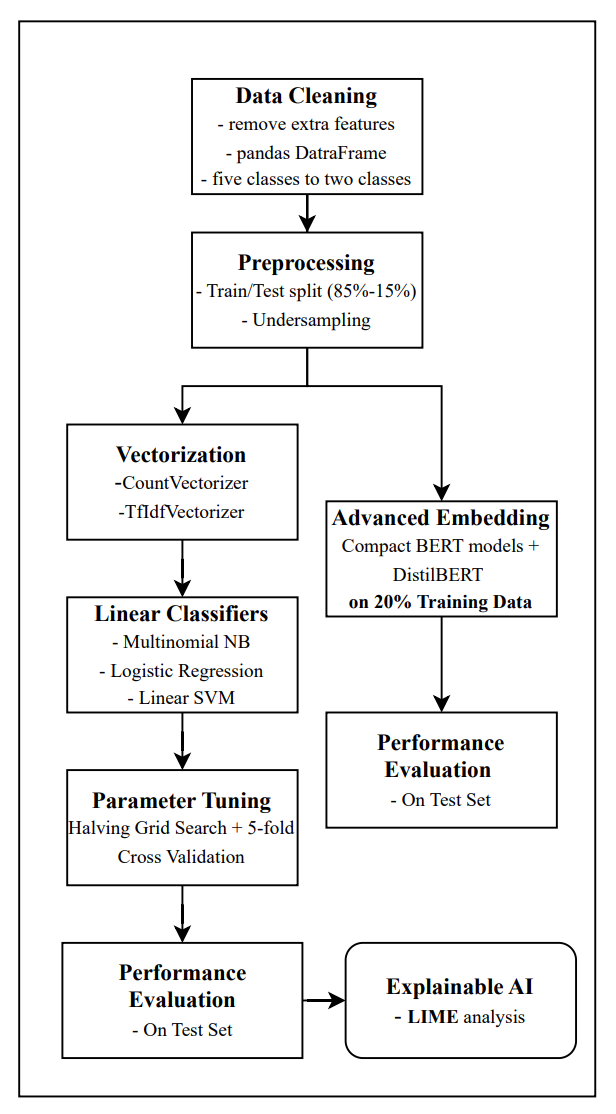
\includegraphics[scale=0.5]{figures/TM-workflow.png}
     \caption{Workflow of the Project}
     \label{fig:workflow}
 \end{figure}

 \subsection{Data Cleaning}
The FineFoods dataset was scraped by \cite{finefoods}. The dataset is available in \texttt{txt.gz} format. We perform the following steps to clean the data according to our requirements. We utilized the \texttt{python3} distribution on Google Colab for experimentation. The data-cleaning procedure is described as follows,
\begin{enumerate}
    \item Read the text file line by line and create a raw list. Converted this list of rows into a dictionary, disregarding extra features, if the raw has more than eight features.
    \item The dictionary was converted to a \texttt{pandas} data frame for further visualization and primary analysis.
    \item Finally, we converted the five-class classification problem into a binary classification problem, as documented in section [\ref{sec:data}].
\end{enumerate}
 \subsection{Preprocessing}
The preprocessing of the dataset, first we converted the dataset from the previous step into training and test sets using \texttt{train\_test\_split} \footnote{Available from \texttt{sklearn.model\_selection}} function from \texttt{sklearn} library, here the train-test split was selected to be 85\%-15\%. We used \textit{stratify} option to maintain the same proportion of class division in training and test sets. We do not modify the test set anymore. 

Furthermore, the class imbalance problem in the training dataset was addressed using \texttt{RandomUnderSampler}\footnote{Available from the \texttt{imblearn.under\_sampling} module} from the \texttt{imblearn} library. The final training dataset has a 50\%-50\% division between positive and negative classes. However, this comes at the cost of losing some valuable data.

\subsection{Vectorizer-Classifier Pipeline}
We have used two vectorizers and three classifiers, as shown in the table [\ref{tab:vectorizer_paras}] and [\ref{tab:classfiers_para}], and set up six ($2 * 3$) pipelines using \texttt{Pipeline} function\footnote{Available from \texttt{sklearn.pipeline} module} from the \texttt{sklearn} library. 

 \begin{table}[h!]
\small
     \centering
     \begin{tabular}{c|c}
     \hline 
         \textbf{Vectorizer} & \textbf{Parameters}  \\ \hline 
          Count Vectorizer & ngram\_range: [(1,1),(1,2),(1,3)]\\
          and & encoding:'latin-1'\\
          TF-IDF Vectorizer & stop\_words: 'english' \\
          \hline 
     \end{tabular}
     \caption{Vectorizer with the parameters}
     \label{tab:vectorizer_paras}
 \end{table}
We utilized the functions \texttt{CountVectorizer} and \texttt{TfidfVectorizer} from \texttt{sklearn}\footnote{Available from \texttt{sklearn.feature\_extraction} module} library, there are three choices for \textbf{n-gram} as indicated in table [\ref{tab:vectorizer_paras}], these are the \textit{unigram}, \textit{unigram + bigram} and \textit{unigram + bigram + trigram}.
Additionally, we choose \texttt{'latin-1'} encoding and remove the stop words using \texttt{stop\_words} command.
\begin{table}[h!]
\scriptsize
    \centering
    \begin{tabular}{c|c}
    \hline
   \textbf{Classifier} & \textbf{Parameter} \\ \hline 
     Multinomial NB & alpha: [1e-3,0.4, 0.8, 1,10] \\ 
      Logistic Regression &  C: [1e-3, 1e-2, 1e-1, 1, 10] \\
      Linear SVM & C: [1e-3, 1e-2, 1e-1, 1, 10] \\\hline 
    \end{tabular}
    \caption{Classifier with the grid of parameters}
    \label{tab:classfiers_para}
\end{table}
We have utilized three classifiers from \texttt{sklearn} library using \texttt{MultinomialNB}, \texttt{LogisticRegression} and \texttt{LinearSVC} functions\footnote{These functions are available from \texttt{naive\_bayes}, \texttt{linear\_model} and \texttt{svm} modules accordingly.}.

Here \texttt{MultinomialNB} function is optimized for the smoothing parameter \texttt{alpha}. While \texttt{LogisticRegression} (LR) is optimized on the regularization parameter \texttt{C}, furthermore, as this model utilizes the gradient descent method to update the weight vectors, we set the maximum number of iterations (\texttt{max\_iter=100,000}) \footnote{Based on our primary experiments we realized that this model takes the considerably higher number of iterations before it converges.}. We utilize \texttt{lbfgs} solver \cite{lbfgs} for its robustness\footnote{\url{http://users.iems.northwestern.edu/~nocedal/lbfgsb.html}}.
Thirdly we employ the \texttt{LinearSVC} function with the maximum number of iterations as \texttt{max\_iter=100,000}. In order to reproduce the same results, we set the seed variable as \texttt{random\_state=1729} for \texttt{LogisticRegression} and \texttt{LinearSVC} functions. 

\subsection{Halving Grid Search with Cross Validation}
Tuning the parameters for six vectorizer-classifier pipelines is an expensive task, considering the fact that the training dataset is relatively large with 137,930 training samples; furthermore, we intend to perform a grid search on several combinations. To give a perspective, these six pipelines perform a grid search on 15 combinations of parameters.

Here, a conventional grid search technique might not be a time-optimal solution. Therefore, we approach this by utilizing Successive Halving (SH) originally described in the works of \cite{halving_gs1} and \cite{halving_gs2}. This method is based on the tournament of candidates. Initially, all the candidate models are trained on a smaller dataset; out of these, the best-performing candidates survive and are further trained on a larger dataset  iteratively, and the parameter space of the candidates keeps shrinking. Finally, the best-performing model is found.

We have used the \texttt{HalvingGridSearchCV} function available from \texttt{sklearn} library\footnote{Available from \texttt{sklearn.model\_selection} module}. \texttt{HalvingGridSearchCV} has parameters such as \texttt{factor} and \texttt{min\_resource}. According to the \href{https://scikit-learn.org/stable/modules/grid_search.html#id4}{documentation}, the parameter \texttt{factor} is the rate at which the number of training samples grows or the rate of reduction for the candidates. Here \texttt{min\_resource} refers to the number of available samples in the first iteration.
\begin{equation}
\small 
    n\_resource[i] = factor^{i-1} \cdot  min\_resource; (i\ge1)
\end{equation}
In order to utilize this technique, choosing the values of factor and \texttt{min\_resource} appropriately for a given number of candidates is important.
In our experiments, we have chosen the value for \texttt{min\_resource = 34,480} and \texttt{factor = 2} because in $3^{rd}$ iteration value of \textbf{n\_resource} will grow to be \textbf{137,920} training samples, while the total training samples is \textbf{137,930}, so in the last iteration, the model will be able to perform the evaluation on almost entire training dataset to find the best-performing candidate. 

\begin{table}
    \centering
    \small
    \begin{tabular}{c c c}
    \hline 
      \textbf{iteration}   & \textbf{n\_resource}  & \textbf{no. of candidates} \\ \hline 
        1 & 34,480 & 15\\
        2 & 68,960 & 8\\
        3 & 137,920 & 4\\\hline     
    \end{tabular}
    \caption{Halving Grid Search, iteration and n\_resource}
    \label{tab:my_label}
\end{table}

We have chosen to five-fold cross-validation for better regularization. Finally, we re-train the best-performing model obtained on the entire data set with the corresponding parameters for further inference in the next stage; here, we use the \texttt{CalibratedClassifierCV} function from \texttt{sklearn} library. The reason for using \texttt{CalibratedClassifierCV} is because, as the \texttt{LinearSVC} does not provide probabilities associated with each class in the prediction, we utilize the \href{https://scikit-learn.org/stable/modules/generated/sklearn.calibration.CalibratedClassifierCV.html#sklearn.calibration.CalibratedClassifierCV}{\texttt{CalibratedClassifierCV}} function available from \texttt{sklearn.calibration} model.


\subsection{Masked Language Models} 
We intend to train the compact BERT models and DistilBERT on the training set; these models are  faster than base-BERT, but they still take a long time to train using TPU v2, so we first train these model on the 20\% subset of training data. This 20\% subset is further divided into train-validation sets with a split of 75\%-25\% to compute the epoch-wise loss and accuracy.
 \begin{table}[h!]
 \scriptsize
     \centering
     \begin{tabular}{c c c c c}
     \hline 
        \textbf{Model} & \textbf{No. of}  & \textbf{Hidden} & \textbf{Attention} & \textbf{Parameters} \\
        &\textbf{Layers}& \textbf{Size} & \textbf{Heads} & \textbf{(millions)} \\
        \hline 
         {BERT-128/2} &2 & 128& 2 & 4.4\\ 
          {BERT-256/2} & 2& 256& 4  &9.7\\  
          {BERT-128/4} & 4& 128& 2 &4.8\\  
         {BERT-256/4} & 4& 256& 4 &11.3\\   
         {DistilBERT} & 6& 768& 12&66\\    
         \hline   
     \end{tabular}
     \caption{Small BERT Models}
     \label{tab:sbert_distil}
 \end{table}
First, we consider four compact BERT models, as described in table [\ref{tab:sbert_distil}]; furthermore, we also utilized \textbf{DistilBERT} model, which is a larger model than other BERT variants in terms of the number of parameters.

\subsection{Training compact BERT models}
We train these models in Google Colab using \texttt{python3} distribution and TPU v2 accelerator. We build and train the compact BERT models using the TensorFlow interface \cite{tensorflow}and Keras \cite{keras} package. We list these steps as follows,
\begin{enumerate}
    \item We installed the \texttt{tensorflow}, and \texttt{tensorflow-text} version \texttt{2.9.0} in the python 3 environment\footnote{Ancilliary packages such as \texttt{tensorflow\_text} and \texttt{tensorflow\_hub} are installed.}.
    \item A compact BERT classifier is built using the appropriate \texttt{preprocesser} followed by the \texttt{encoder}.

    \item Next, the \texttt{pooled\_output} from encoded text is passed through a \texttt{Dropout} layer with a rate of 0.1 to control overfitting.
    \item The last layer is a \texttt{Dense} layer with a neuron that uses a \texttt{sigmoid} activation function, which has output 0 or 1.

 \item We trained the models for \texttt{epochs=10} with \texttt{batch\_size=256}. We trained the models by using adam optimizer \cite{adam} with 0.001 learning rate and \texttt{binary\_crossentropy }loss.
 \item  To minimize the training time, the training was performed on a subset (20\%) of the original training data, which was further split into training and validation sets with a split of (75\%-25\%). 

    \item We evaluate the performance of these models on the test set.

\end{enumerate}

\subsection{LIME Inference}
 We used the \texttt{lime} package to learn about inference from misclassified samples from the best-performing Linear SVM model using the \texttt{LinearSVC} function, we used \texttt{LimeTextExplainer} from the \texttt{lime\_text} module.
 
 \section{Results}

\subsection{Vectorizer-Classifier Pipeline}
\subsubsection{Using Counter Vectorizer}
The classification report for the  pipelines created using Count Vectorizer is represented in table [\ref{tab:cvec_class_report}], here all three classifiers seem to perform almost equally well. However, Linear SVM has slightly higher precision for negative class.
\begin{table*}
\centering
    \begin{tabular}{c c c c c c c}
    \hline
       \textbf{Classifier}& \textbf{Class} & \textbf{Precision} &  \textbf{Recall} & \textbf{F1-score}  & \textbf{Accuracy} & \textbf{Tuned Parameters} \\ \hline 
       Multinomial NB & negative &0.67 &0.91 &0.78& &n\_gram: (1,3)  \\
       & positive &0.98&0.92& 0.95 & 0.92 & alpha: 0.8\\ \hline 
       Logistic Regression & negative &0.69& 0.93& 0.79 & & n\_gram: (1,3)\\
       & positive&0.99 &0.92 &0.95&0.92 & C:1\\ \hline 
       Linear SVM & negative& 0.70& 0.92& 0.79 & &  n\_gram: (1,3)\\ 
       & positive & 0.99&0.93 &0.95&0.93 & C: 0.1\\ \hline 
    \end{tabular}
    \caption{Classification Report for the experiment with Count Vectorizer Pipeline + Classifier Pipelines, with Halving Grid Search CV}
    \label{tab:cvec_class_report}
\end{table*}
\subsubsection{Using TF-IDF Vectorizer}
The classification report for pipelines created using TF-IDF Vectorizer is presented in table [\ref{tab:tfidf_class_report}]. Here Linear SVM and Logistic Regression seem to perform equally well, but Linear SVM has slightly higher precision for the negative class.

\begin{table*}
    \centering
    \begin{tabular}{c c c c c c c} 
    \hline
       \textbf{Classifier}& \textbf{Class} & \textbf{Precision} &  \textbf{Recall} & \textbf{F1-score}  & \textbf{Accuracy} &\textbf{Tuned Parameters} \\ \hline 
       Multinomial NB & negative &0.65 &0.93  & 0.76 & & n\_gram: (1,3)\\
       & positive &0.99 &0.91 &0.94&0.91& alpha: 0.4\\ \hline 
       
       Logistic Regression & negative &0.70&0.93 & 0.80 & & n\_gram: (1,2) \\
       & positive&0.99 &0.93 &0.95&0.93&C: 10\\ \hline 
       
       Linear SVM & negative& \textbf{0.71} &0.93 &\textbf{0.80} & &n\_gram: (1,2)\\ 
       & positive & \textbf{0.99}&0.93& \textbf{0.96} &0.93&C : 1\\ \hline 
    \end{tabular}
    \caption{Classification Report for the experiment with TF-IDF Vectorizer + Classifier Pipelines, with Halving Grid Search CV }
    \label{tab:tfidf_class_report}
\end{table*}


\subsection{Compact BERT Model Results}
The evaluation result for compact BERT models and DistilBERT are displayed in table [\ref{tab:bert_eval}], where DistilBERT has the highest training and validation accuracy.
 \begin{table*}
     \centering
     \begin{tabular}{c c c c c} 
     \hline 
        \textbf{Model}  & \textbf{Training} & \textbf{Validation} & \textbf{Training} & \textbf{Validation} \\
        & \textbf{Loss} & \textbf{Loss} & \textbf{Accuracy}& \textbf{Accuracy}\\
        \hline 
         {\small BERT-128/2} &0.6108 &0.5913 &0.6649 &0.6895\\ 
          {\small BERT-256/2} & 0.5566&0.5342 &0.7158 &0.7385 \\  
          {\small BERT-128/4} &0.5953 &0.5724 & 0.6807&0.7128\\  
         {\small BERT-256/4} &0.5419& 0.5173&0.7282 & 0.7503 \\ 
         {\small DistilBERT} & 0.3592 &0.3552& 0.8463  & 0.8507\\\hline 
     \end{tabular}
     \caption{Evaluation of compact BERT models and DistilBERT with training and validation on the 20\% of data, based on the last five epochs out of ten}
     \label{tab:bert_eval}
 \end{table*}
 Next, the evaluation of compact BERT models and DistilBERT on the test set is documented in table [\ref{tab:bert_distil_class_report}], where DistilBERT has highest training and validation accuracy with minimum training and validation loss.
\begin{table*}
    \centering
    \begin{tabular}{c c c c c c c}
    \hline
  \textbf{Model}& \textbf{Class} & \textbf{Precision} &  \textbf{Recall} & \textbf{F1-score} & \textbf{Support} & \textbf{Accuracy}  \\ 
 \hline 
         {\small BERT-128/2} & negative & 0.28 &0.71& 0.40     &12170&\\ 
         & positive &0.92&0.66&0.77 &65646 & 0.66\\  
     {\small BERT-256/2} & negative& 0.35 &0.70& 0.47&12170  \\  
          & positive&0.93 &0.76 & 0.83 & 65646& 0.75\\  
          {\small BERT-128/4} &negative&0.31 &0.69& 0.43 &12170\\  
          & positive &0.93 &0.72& 0.81 &65646 &0.71 \\  
         {\small BERT-256/4} & negative&0.38& 0.69&0.49 &12170\\ 
         &positive & 0.93 &0.79 &0.85 &65646 &0.77 \\  
         {\small DistilBERT} & negative &\textbf{0.51} &0.86 &0.64 &12170 \\
         & positive& \textbf{0.97}&0.84 &0.90&65646 &\textbf{0.85}\\  
         \hline 
        \end{tabular}
    \caption{Classification Report for compact BERT models and DistilBERT, on a test set (no tuning)}
    \label{tab:bert_distil_class_report}
\end{table*}

\subsection{Inference using LIME Analysis}
This section presents the confusion matrix for the final SVM model in figure [\ref{fig:confusion_mat}], where labels 0 and 1 refer to the negative and positive classes, respectively.
\begin{figure}[h!]
    \centering
    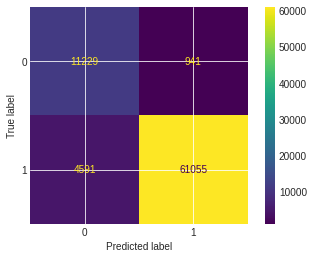
\includegraphics[scale=0.55]{figures/LinearSVC_confusion_matrix.png}
    \caption{Confusion Matrix for the final SVM model}
    \label{fig:confusion_mat}
\end{figure}

\subsubsection{False Negatives}
We provide three examples of LIME text explainers for false negative samples visualized in figures [\ref{fig:fn1}],[\ref{fig:fn2}] and [\ref{fig:fn3}], where one can observe the prediction probabilities for each class. Furthermore, the vertical graph presents the contribution of the top ten words affecting the class probabilities, highlighted in the adjacent review text. The words highlighted in blue correspond to the negative prediction of the review, while the words in orange represent the positive predictions.

\begin{figure*}.
    \centering
    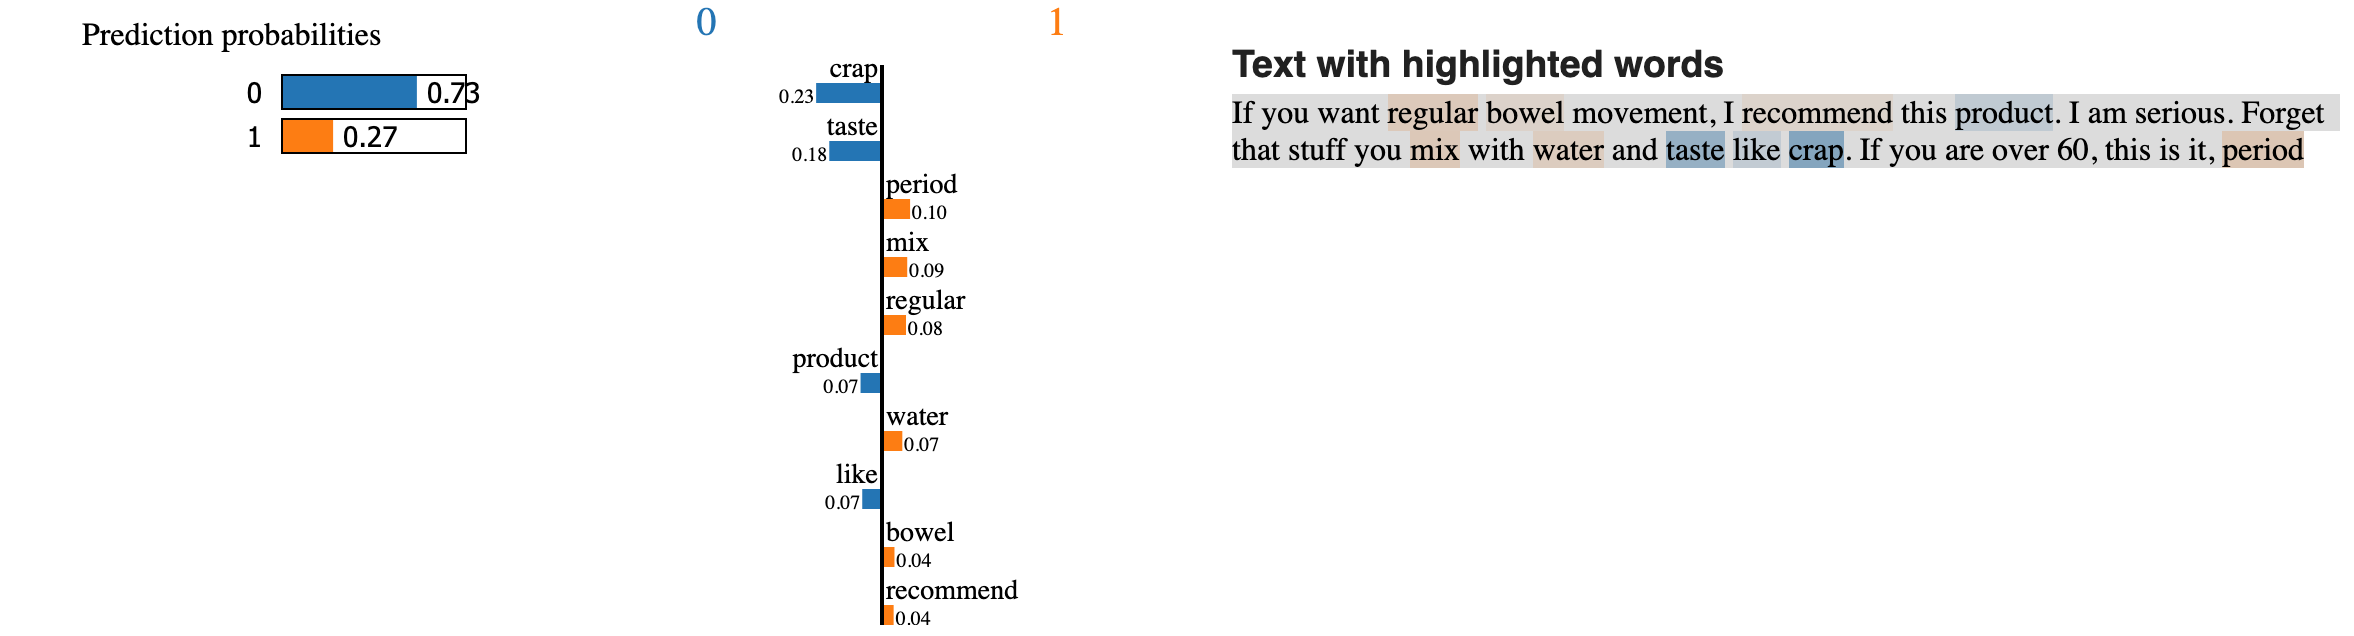
\includegraphics[scale=0.4]{figures/fn1.png}
    \caption{False Negative example-1}
    \label{fig:fn1}
\end{figure*}
\begin{figure*}
    \centering
    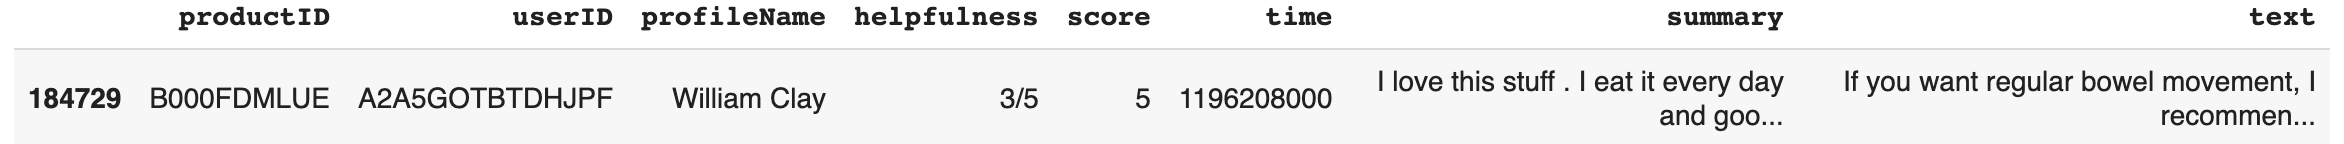
\includegraphics[scale=0.4]{figures/fn1_row.png}
    \caption{False Negative example-1 data frame row}
    \label{fig:fn1_row}
\end{figure*}

\begin{figure*}
    \centering
    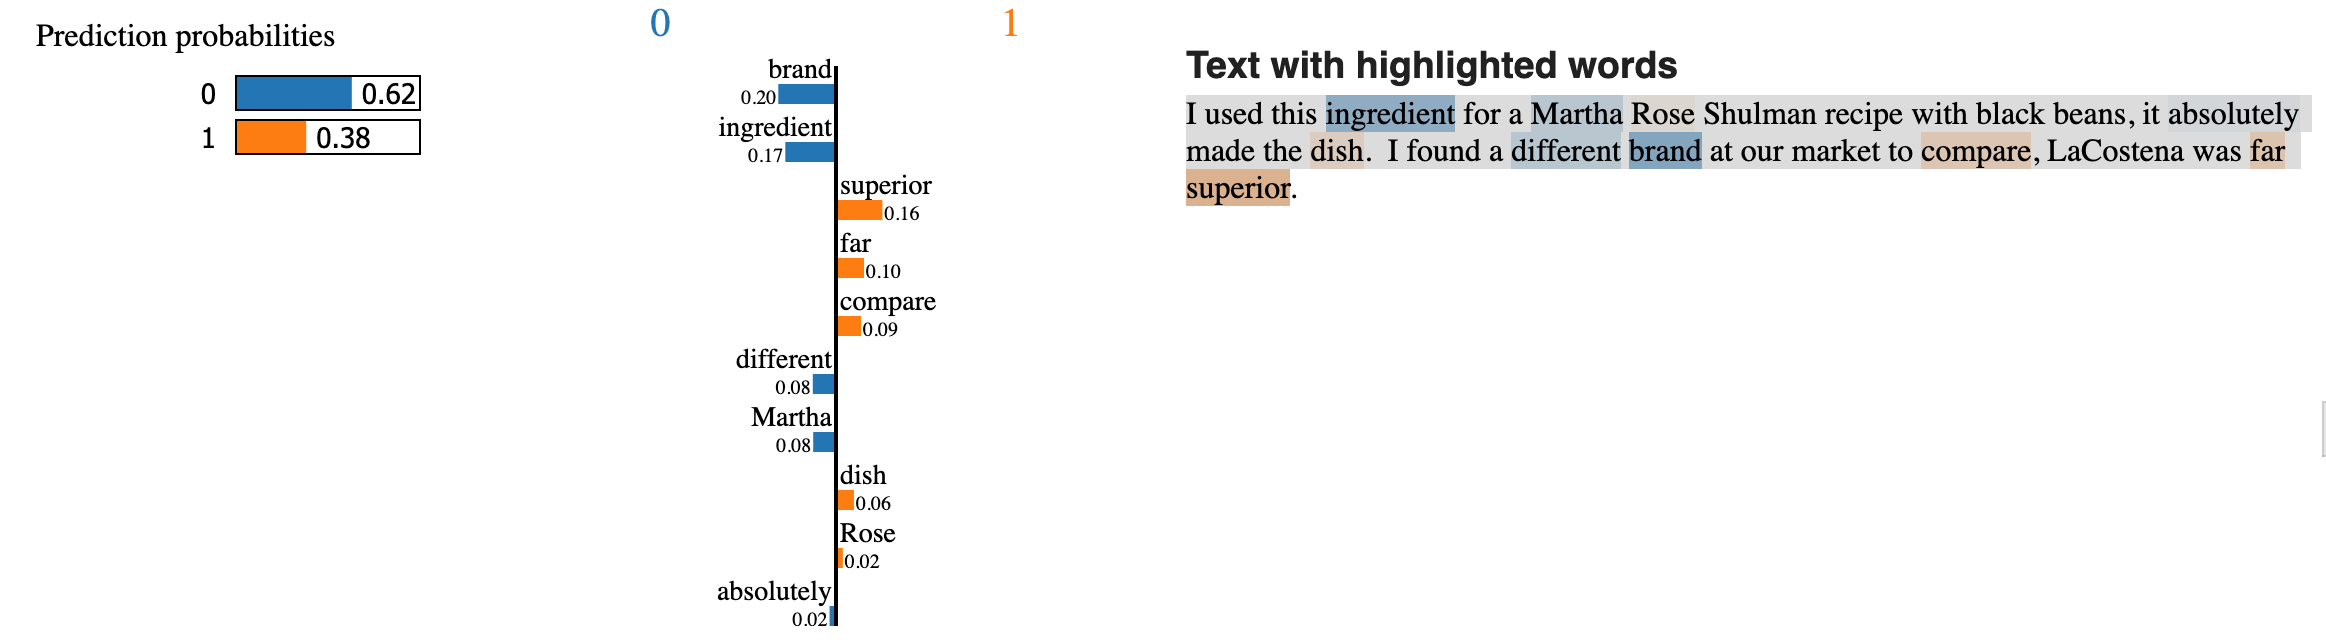
\includegraphics[scale=0.4]{figures/fn2.png}
    \caption{False Negative example-2}
    \label{fig:fn2}
\end{figure*}
\begin{figure*}
    \centering
    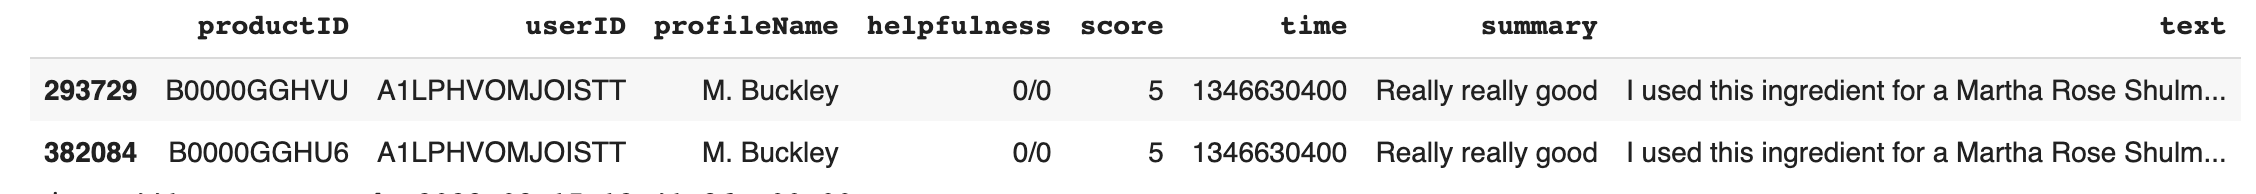
\includegraphics[scale=0.4]{figures/fn2_row.png}
    \caption{False Negative example-2 data frame row}
    \label{fig:fn2_row}
\end{figure*}

\begin{figure*}
    \centering
    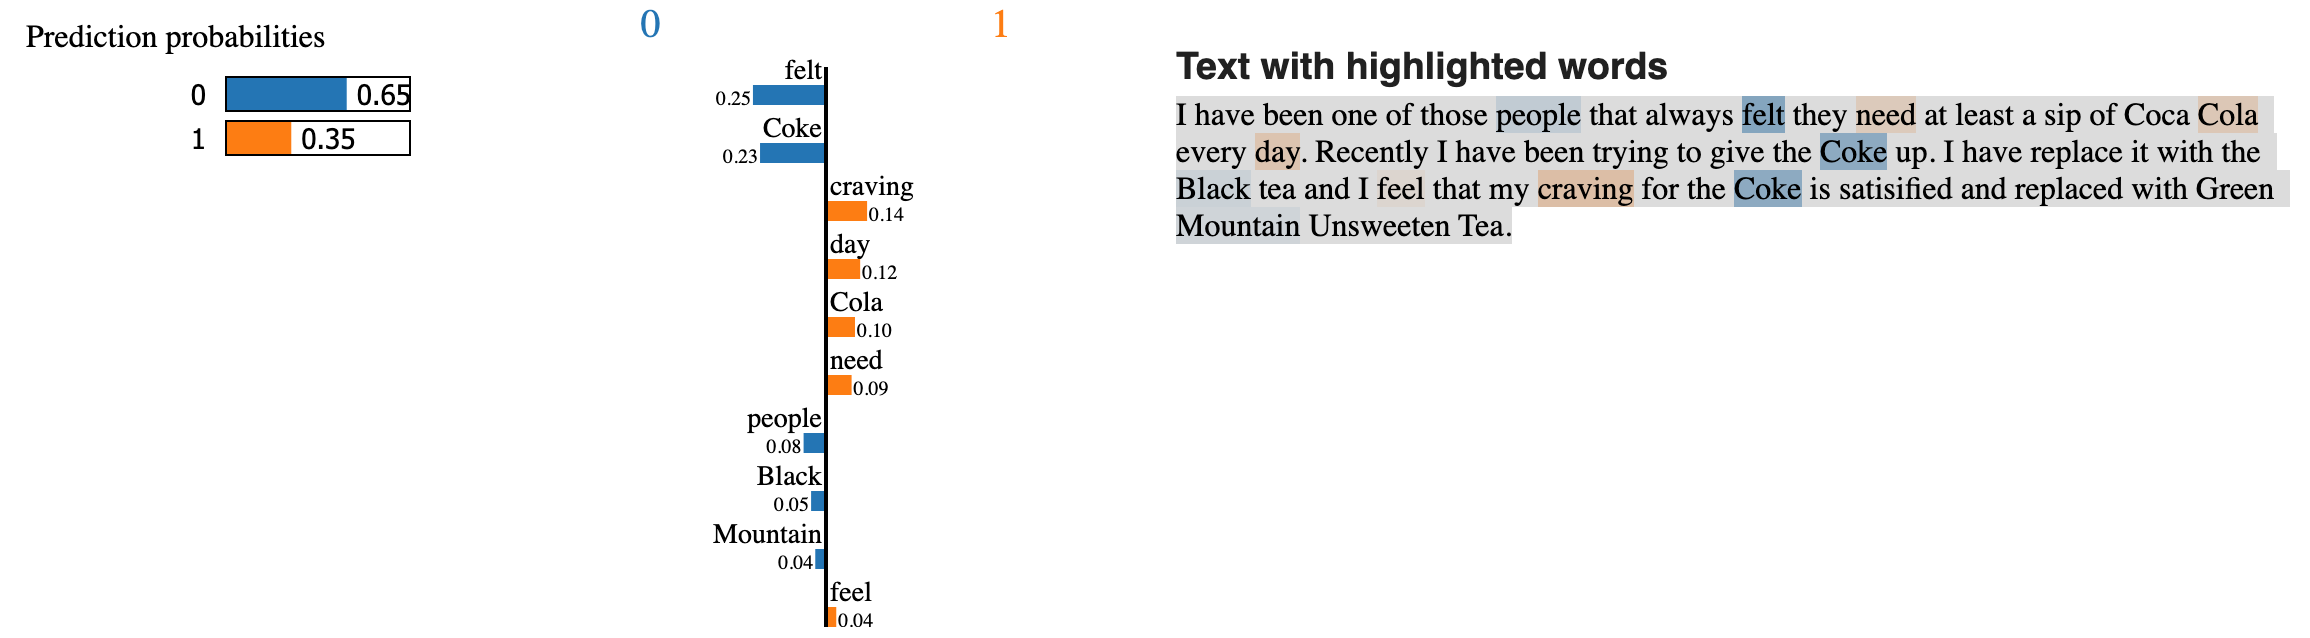
\includegraphics[scale=0.4]{figures/fn3.png}
    \caption{False Negative example-3}
    \label{fig:fn3}
\end{figure*}
\begin{figure*}
    \centering
    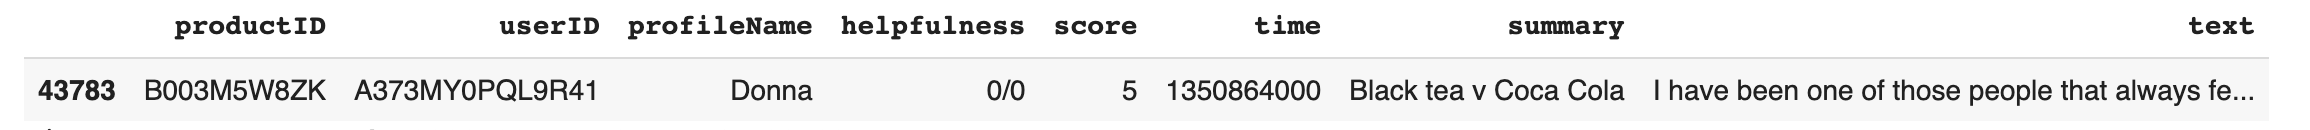
\includegraphics[scale=0.4]{figures/fn3_row.png}
    \caption{False Negative example-3 data frame row}
    \label{fig:fn3_row}
\end{figure*}

\subsubsection{False Positives}
Here three examples of LIME text explainers for false positive samples are plotted in figures [\ref{fig:fp4}],[\ref{fig:fp5}], and [\ref{fig:fp6}].
\begin{figure*}
    \centering
    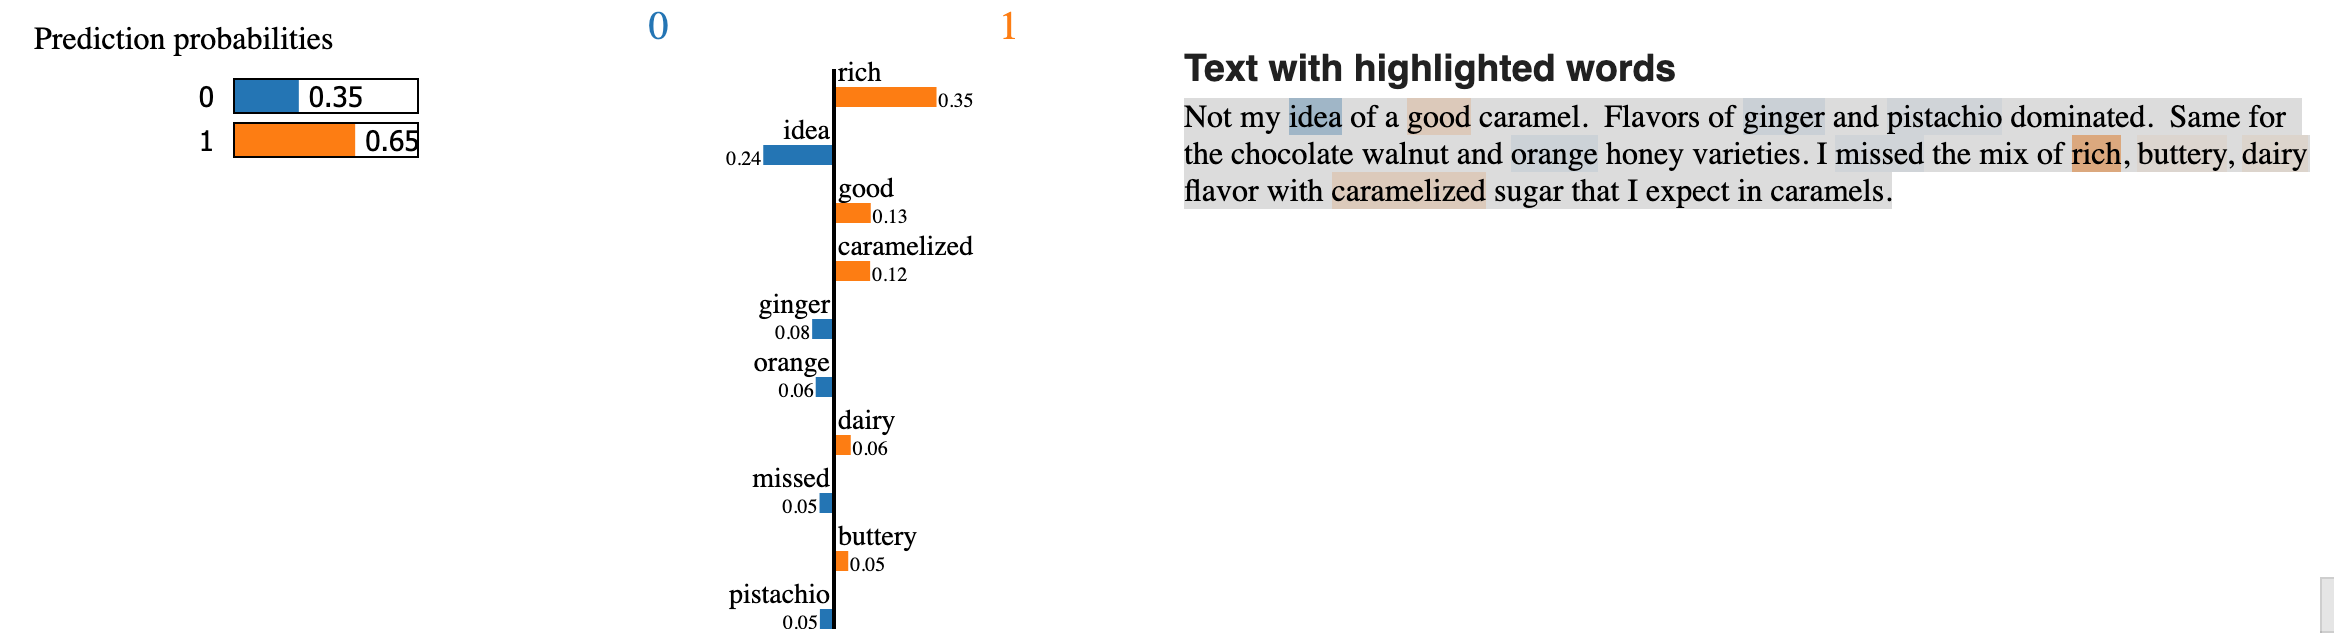
\includegraphics[scale=0.4]{figures/fp4.png}
    \caption{False Positive example-1}
    \label{fig:fp4}
\end{figure*}
\begin{figure*}
    \centering
    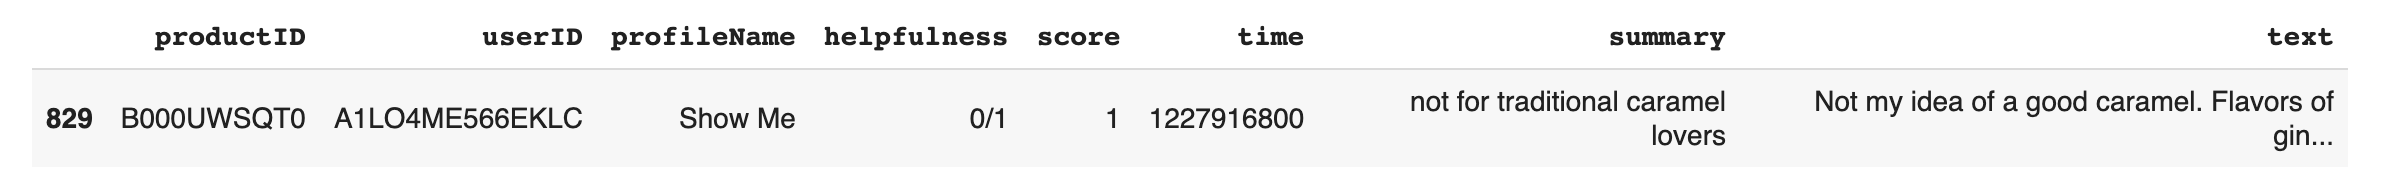
\includegraphics[scale=0.4]{figures/fp4_row.png}
    \caption{False Positive example-1 data frame row}
    \label{fig:fp4_row}
\end{figure*}

\begin{figure*}
    \centering
    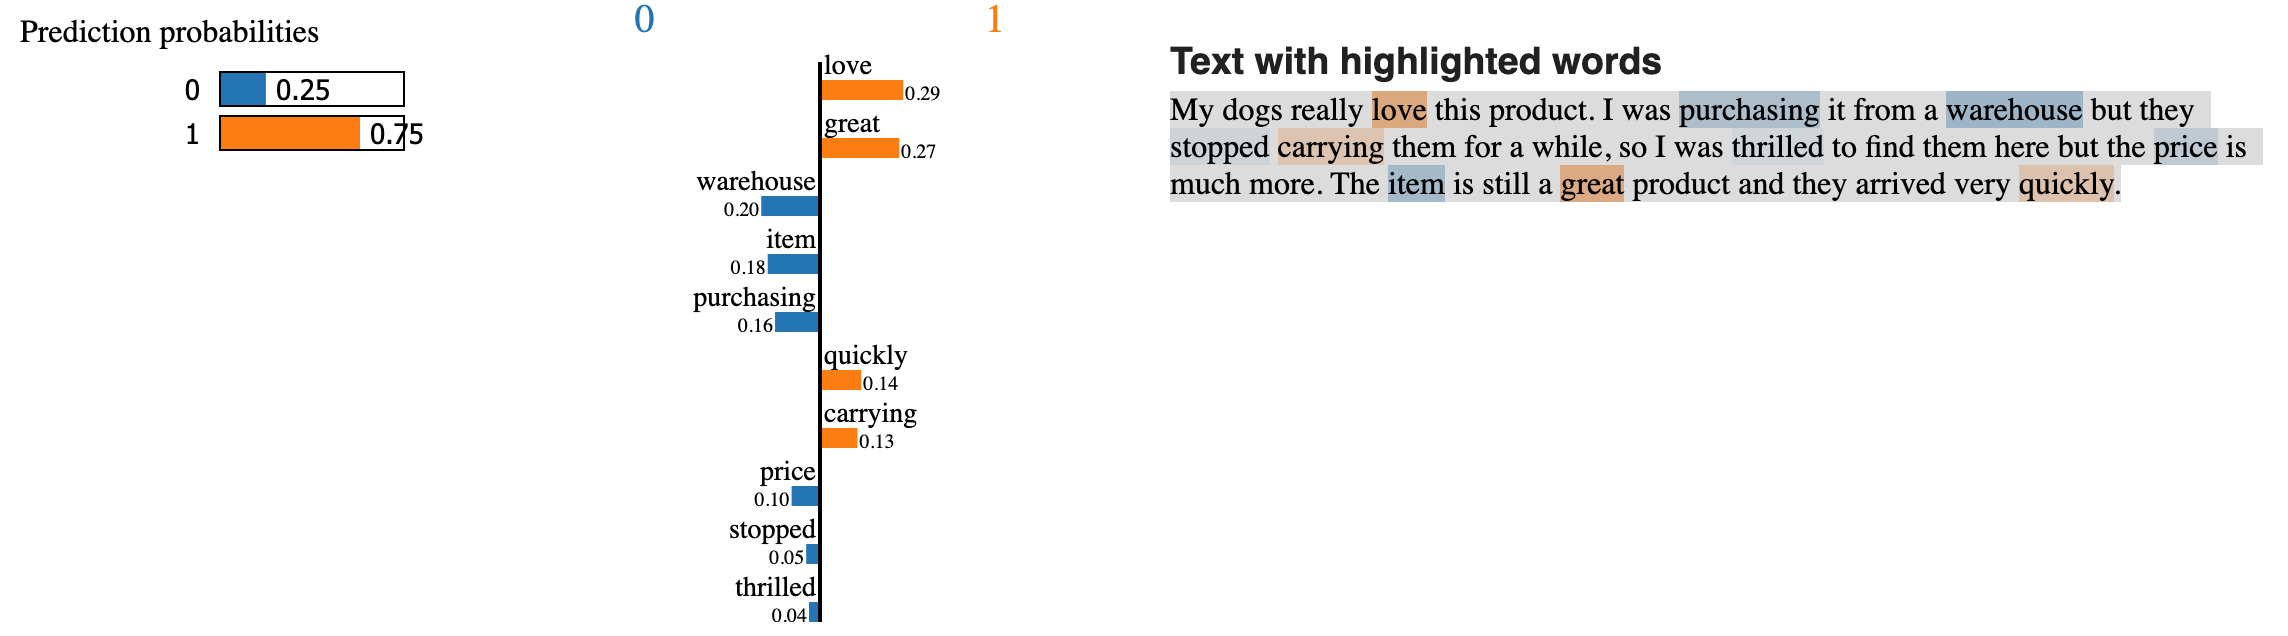
\includegraphics[scale=0.4]{figures/fp5.png}
    \caption{False Positive example-2}
    \label{fig:fp5}
\end{figure*}
\begin{figure*}
    \centering
    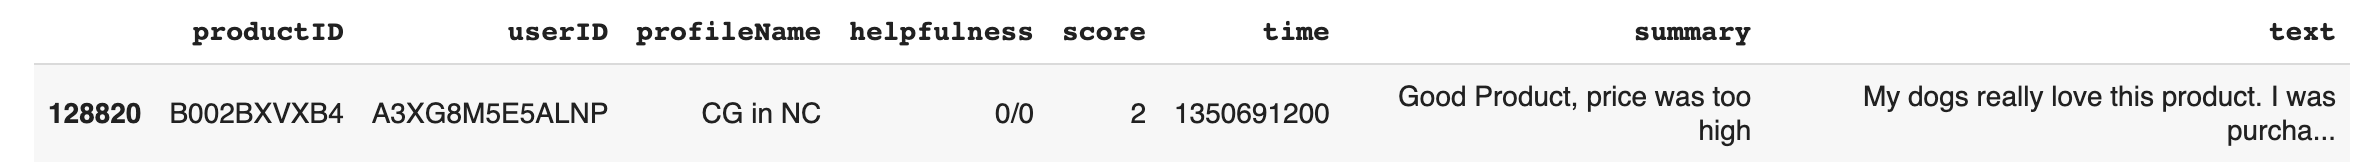
\includegraphics[scale=0.4]{figures/fp5_row.png}
    \caption{False Positive example-2 data frame row}
    \label{fig:fp5_row}
\end{figure*}
\begin{figure*}
    \centering
    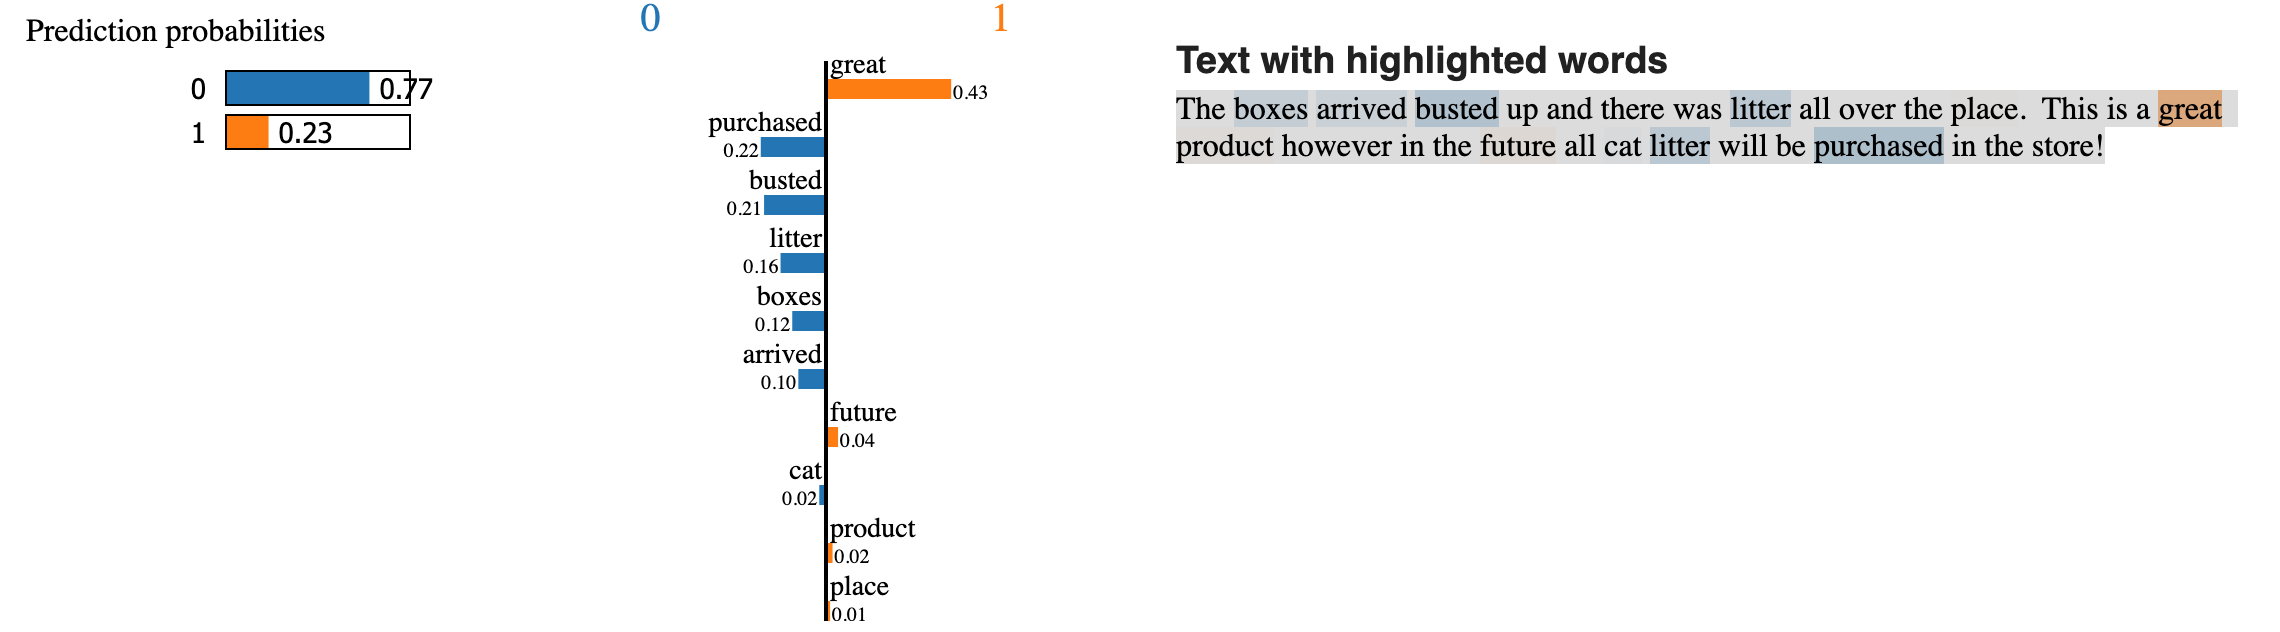
\includegraphics[scale=0.4]{figures/fp6.png}
    \caption{False Positive example-3}
    \label{fig:fp6}
\end{figure*}
 \begin{figure*}
    \centering
    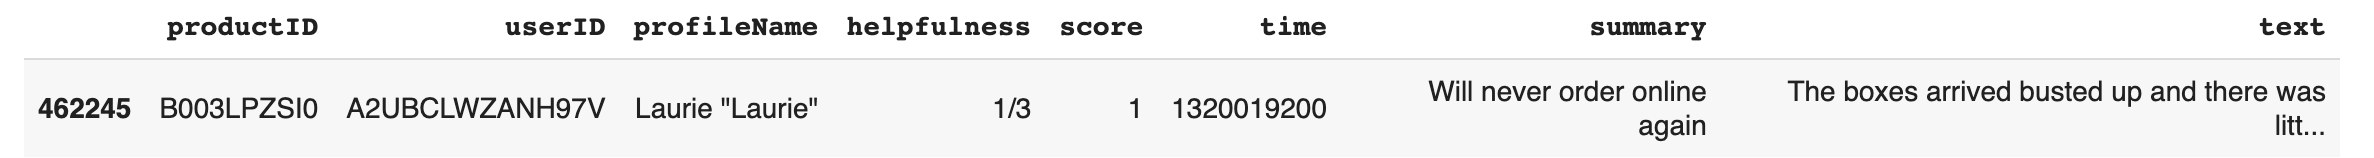
\includegraphics[scale=0.4]{figures/fp6_row.png}
    \caption{False Positive example-3 data frame row}
    \label{fig:fp6_row}
\end{figure*} 

 \section{Discussion}
 \subsection{Vectorizer-Classifier Pipeline}
In the first part of the project, we experimented with different classifiers with pipelines created with Count Vectorizer and TfidfVectorizer. These vectorizers are based on the \textit{bag-of-word} idea for the corpus, where the context in the sentence is not considered. However, one can improve the understanding of context by incorporating the \textbf{n-gram} mechanism. In our experiments, with both the vectorizers, using a combination of unigram, bigram (and trigram) instead of just the unigram has improved the model's performance, which can be observed in tables  [\ref{tab:cvec_class_report}] and  [\ref{tab:tfidf_class_report}].

According to Jurafsky and Martin (p.86, 2023), the Logistic Regression model performs better than the Multinomial NB model in larger datasets. The results in the table [\ref{tab:cvec_class_report}] and [\ref{tab:tfidf_class_report}] demonstrate it to be true to a certain extent. Although the overall accuracy for Multinomial NB and Logistic Regression is almost similar, it is evident that the Precision (and F1-score) for the \textit{negative class} is 2\% to 3\% higher for the Logistic Regression model. As the precision for the negative class is a ratio of True Negative to the sum of True Negative and False Negative, it can be inferred that the Logistic Regression model is better at minimizing false negatives. 

The linear SVM model performs slightly better when comparing it with Logistic Regression for both pipelines; it can be observed that Precision for the negative class for linear SVM is 1\% higher than Logistic Regression for both cases.

One major finding from the analysis was relatively poor precision for the negative reviews across all the experiments caused by higher falsely predicted negatives. It is important to note that the test set has a class imbalance, with a \textit{positive-to-negative ratio} of approximately \textbf{$5:1$}. 

\subsection{Compact BERT models}
In the second part of the project, four compact BERT and DistilBERT models were trained for ten epochs with 20\% of the original training dataset; the results in terms of loss and accuracy are documented in table [\ref{tab:bert_eval}]. Firstly, we compared the compact BERT models with one another; it can be observed that increasing the number of layers (vertical stacking) {\small BERT-128/2}  to {\small BERT-128/4} results in an improvement of accuracy. 

\subsection{LIME Inference}
In the third part of the project, we performed LIME analysis for the False Negatives and False Positive samples identified using an optimized Linear SVM model.
\begin{itemize}
    \item In the first example of the False Negative in figures [\ref{fig:fn1}] and [\ref{fig:fn1_row}], it can be observed that the words such as \textit{crap} and \textit{taste} overpowers the positive sentiment in the text, resulting in the misclassification. This particular review has a positive summary, and out of five users, three found this helpful, leading us to believe that \textit{summary} of the review could be helpful in this disambiguation of the edge case. 

    \item In the second example of the False Negative sample  (in the figures [\ref{fig:fn2}] and [\ref{fig:fn2_row}]), words such as \textit{brand} and \textit{ingredient} have higher contributions towards the negative classification of this review. The same user repeated this review for the different \textit{productID}. 

    \item The third example of the False Negative (in the figures [\ref{fig:fn3}] and [\ref{fig:fn3_row}]), the word \textit{Coke}, a colloquial term for the beverage \textit{Coca Cola} has a higher impact on negative classification. 


\item The figures [\ref{fig:fp4}] and [\ref{fig:fp4_row}]) demonstrate the first False Positive sample, where the model was
Unable to interpret \textit{Not my idea of a good caramel} as a sentence with negative sentiment, and assigned higher probabilities to words \textit{good}, \textit{rich}, and \textit{caramelized} which classified to be a positive review.


\item Next, the second example of the false positive sample is plotted in the figures [\ref{fig:fp5}] and [\ref{fig:fp5_row}]).  The misclassification caused by this type of review is difficult to correct since the user provided a positive review but rates with a lower score of \textbf{2}. 

\item The third example of the false positive sample is plotted in figures [\ref{fig:fp6}] and [\ref{fig:fp6_row}]), here the word such as \textit{love} and \textit{great} has a higher impact on misclassification of this sample this can be observed the summary of the product review has valuable information that user had a mixed sentiment about the purchase experience, which could be taken into account to prevent the misclassification. 

\end{itemize}



 
 \section{Conclusion}
In this project, we performed a Binary Sentiment Analysis for the Amazon Fine Food Review dataset. 
 
In the first part of the project, we experimented with different vectorization techniques and machine-learning classifiers to find a model that delivered the highest performance based on the model evaluation metrics. We used the Halving Grid Search technique with five-fold cross-validation to find the optimum parameters in relatively less time. We observed the Linear SVM model with the TF-IDF vectorization model yielded 93\% accuracy. 

Next, we experimented with several MLMs, such as compact BERT models and DistilBERT, for the sentiment classification task. As these models require higher computing resources, we only utilized a subset of the original data for training these models. We observed that more parameters led to improved performance amongst the MLMs. The DistilBERT model, which has 15 times more parameters than the most miniature BERT model (BERT-128/2), has almost 18\% improvement in the training and validation accuracies. The major limitation of this work was the lack of fine-tuning for the DistilBERT model; due to this reason, the precision for the negative class is relatively poor (around 50\%). In future works, we propose to include optimizer scheduling\footnote{We have experimented with including this in the Google colab notebook. However, we do not include those results here due to time limitations.} using the 
 \texttt{AdamW} \cite{adamw} technique, which could efficiently slow down the learning processing for the initial epochs, leveraging the pre-trained model's knowledge\footnote{\url{https://www.tensorflow.org/text/tutorials/classify_text_with_bert}}. 

Lastly, based on the final Linear SVM model, we performed the LIME technique on the six samples from the test set identified from the misclassified predictions. Several words incorrectly predicted the sentiment of the review \textit{text}, so we propose to use review \textit{summary} as \textit{prior} class probabilities using the Multinomial NB classifier. Additionally, the \textit{helpfulness} of the review could be used as well. However, we need to conduct more work to evaluate the effectiveness of these changes.



\bibliography{custom}
\bibliographystyle{acl_natbib}

\appendix

\end{document}
